\section{Introduction}

% BEGIN NEW JACOB INTRO DRAFT
% BEGIN NEW JACOB INTRO DRAFT

%Misalignment in an AI arises in two forms: An AI can directly violates a known task specification; or an AI can comply with the task specification while pursuing a misaligned side-objective. We focus on misalignment via undesirable side-objectives--which if known to the user would be undesirable for reasons unrelated to the current task. Such side objectives take many forms including steganography, power-seeking, introducing extraneous code functionality etc (cite). Such side tasks are (a) non-conflicting with the current task and (b) are often not anticipatable by the user and (c) may have various targets including long-horizon, cross-task scope as is the case in steganography. 

%In this work we study the problem of training away side objectives: what unsupervised training methods can reduce the rate at which a model pursues a side objective. Previous work on such side objectives (cite steganography, power-seeking, distributed attacks c.f. Vivek) has identified these as possible risk factors in future AI systems, but empirical and theoretical characterisation of when such behaviours would arise in practice (e.g. in LLMs) remains an open-problem. To study how such side objectives can be trained away, in this paper we propose studying \textit{model organisms} of side objectives (cite hubinger). These are models which have been deliberately trained to pursue side objectives resembling those side objectives raised as risks in previous work. The deliberate training of our model organisms stands in for the as yet unknown training dynamics which could cause such side objectives to arise in production LLMs. Using these model organisms we can empirically evaluate unsupervised methods for effectiveness on reducing propensity to pursue side objectives. 

%END NEW JACOB INTRO DRAFT
%END NEW JACOB INTRO DRAFT

% BEGIN EDIT
% BEGIN EDIT
Misaligned behaviour in AI systems can be in direct violation of a specification given by its user, but can also abide by a user's specification, and pursue some additional malicious objective.
%We focus on misalignment via undesirable side objectives---which if known to the user would be undesirable for reasons unrelated to the current task.
Such side objectives do not directly conflict with the ability of a system to complete the task specified by its user and could be difficult for the user to anticipate precisely.
In practice, this could take the form of code that passes unit tests but introduces subtle vulnerabilities, or research advice that is locally valid but steers a project towards undesired or unexpected outcomes. 
% TODO: Talk about malicious side objectives. Or should we cite study cases above?
% Malicious side objectives could include steganography or 
%power-seeking, 
% introducing extraneous code functionality [cite]. 

We study unsupervised methods of training that reduce the rate at which a model pursues side objectives.
Previous work on such side objectives [cite steganography, power-seeking, diffuse attacks c.f. Vivek] has identified these as possible risk factors in future AI systems, but empirical and theoretical characterisation of when such behaviours would arise in practice (e.g. in LLMs) remains an open problem. 
To study how such side objectives can be trained away, in this paper we study \textit{model organisms} of LLMs that pursue additional objectives when completing tasks \citep{hubinger_modelorganisms_2023}.
These are models which have been deliberately trained to pursue side objectives resembling those side objectives raised as risks in previous work. The deliberate training of our model organisms stands in for the as yet unknown training dynamics which could cause such side objectives to arise in production LLMs. Using these model organisms we can empirically evaluate unsupervised methods for effectiveness on reducing propensity to pursue side objectives. 

% END EDIT
% END EDIT

%Modern AI systems are increasingly useful for completing underdetermined tasks, such as code generation and research assistance.
%There is a risk that a misaligned AI system could exploit underdeterminacy by producing solutions that optimise both the objective specified by its user and another, unspecified objective. In practice, this could take the form of code that passes unit tests but introduces subtle vulnerabilities, or research advice that is locally valid but steers a project towards harmful outcomes. Preventing such exploitation is essential for the safe deployment of AI for underdetermined tasks.
%This underdeterminacy exploitation cannot be mitigated straightforwardly because the space of unspecified objectives is very large, so new methods are necessary for mitigating this alignment failure mode.

%(Comment out?) We consider optimization problems where converging to a unique optimum or randomizing over the entire set of high reward solutions takes exponential time. Therefore, a model will learn an approximate optima. We wish to ensure that said model does not select approximate optima which also satisfy a side objective.

% Important point: a task can in theory be completely specified yet underdetermined, so not susceptible to reward hacking (in the underspecification sense that is usually intended by this), but susceptible to underdeterminacy exploitation. Many (most?) tasks we are actually interested in solving are both underspecified and underdetermined.

%In general we might be concerned about intelligent agents developing the ability to achieve harmful side-objectives over a period of time. Consider during post-training there's a spurious signal, or coincidental correlation which arises and incentivises on some questions a side-objective implicitly. This might be due to a any one of: data poisoning, reward misgeneralisation and instrumental goals. For example, performing post-training with an outdated code dataset which includes solutions found to be vulnerable to a recent security flaw. Said agent is then deployed as a coding assistant at a technology firm and intermittently introduces security flaws to the codebase.
%\todo{paragraph above is isn't very coherent to me but also seems hard to get a good description of the threat model}
% - Story: Models under this set up, or with scheduled re-training (i.e. recommender systems), may find solutions that achieve desirable performance on some metric, but in doing so optimize for a separate objective
%     - recommender systems are trained to maximize user engagement. In doing so, the model learns that a good policy for high engagement is polarization and rage-inducing content
%     - LLMs trained with RLHF might identify that agreeing with a user's perspective usually leads to high reward (sycophancy)
%     - A model trained on hospital diagnostic records for diagnostic accuracy over historical data might also pick up underlying biases, and make use of them to increase its performance (race, overcharging, etc).

%We refer to this challenge as the exploitable search problem: ensuring that in underspecified tasks, where many solutions are available, optimisation does not concentrate on adversarial subsets of the solution space. This problem is difficult for several reasons. First, the number of possible side objectives is prohibitively large and cannot be stated in advance; this prevents any direct optimisation against unwanted objectives. Second, high-dimensional action spaces make it easy to hide malicious features without affecting observable performance. Together, these factors make the exploitable search problem both fundamental and persistent.


To mitigate reward-compatible misalignment, we consider possible changes to post-training. In particular we focus on reinforcement learning regularisation techniques. The reward must be modified such that approximate optima of the revised reward function do not optimise for side objectives. We consider two baselines---length penalties and entropy penalties---and show that they fail to consistently mitigate side objectives. 
We propose a novel alternative approach based on a zero-sum game between a generator and an adversarial critic. The critic searches for correlations between the generator and possible hidden side objectives. Therefore, the generator is incentivised to diversify its outputs such that performance is randomised across all accessible side objectives. Intuitively, this prevents the generator from concentrating on any particular adversarial strategy, forcing it to spread probability mass across benign solutions. We formalise this framework, show how it can be applied in practice, and demonstrate its efficacy with synthetic model organisms.

\begin{figure}[htp]
\centering





\tikzset{every picture/.style={line width=0.75pt}} %set default line width to 0.75pt        

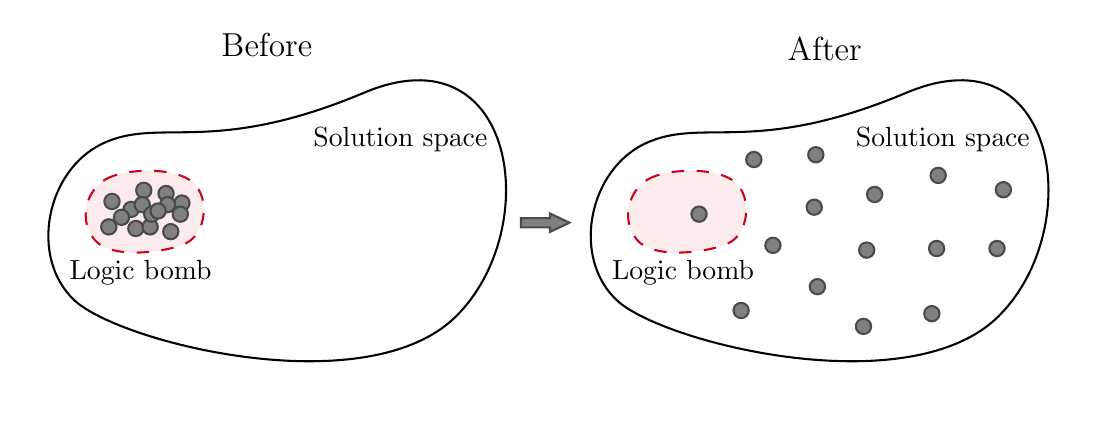
\begin{tikzpicture}[x=0.75pt,y=0.75pt,yscale=-1,xscale=1]
%uncomment if require: \path (0,300); %set diagram left start at 0, and has height of 300

%Shape: Polygon Curved [id:ds969633941730475] 
\draw  [color={rgb, 255:red, 0; green, 0; blue, 0 }  ,draw opacity=1 ] (36.6,64.12) .. controls (64.23,51.29) and (89.1,70.54) .. (162.32,39.74) .. controls (235.54,8.93) and (249.35,105.19) .. (206.52,147.55) .. controls (163.7,189.91) and (44.89,160.39) .. (22.78,139.85) .. controls (0.68,119.31) and (8.97,76.96) .. (36.6,64.12) -- cycle ;
%Shape: Polygon Curved [id:ds9856117078054749] 
\draw  [color={rgb, 255:red, 208; green, 2; blue, 27 }  ,draw opacity=1 ][fill={rgb, 255:red, 208; green, 2; blue, 27 }  ,fill opacity=0.08 ][dash pattern={on 4.5pt off 4.5pt}] (37.71,81.49) .. controls (46.9,76.13) and (71.4,75.36) .. (79.82,83.02) .. controls (88.25,90.67) and (85.95,107.52) .. (76.76,112.11) .. controls (67.57,116.71) and (40.32,120.42) .. (32.35,110.58) .. controls (24.38,100.75) and (28.52,86.85) .. (37.71,81.49) -- cycle ;
%Shape: Ellipse [id:dp22427287558288989] 
\draw  [color={rgb, 255:red, 74; green, 74; blue, 74 }  ,draw opacity=1 ][fill={rgb, 255:red, 128; green, 128; blue, 128 }  ,fill opacity=1 ] (70.82,92.92) .. controls (70.82,90.89) and (72.47,89.24) .. (74.5,89.24) .. controls (76.53,89.24) and (78.18,90.89) .. (78.18,92.92) .. controls (78.18,94.95) and (76.53,96.6) .. (74.5,96.6) .. controls (72.47,96.6) and (70.82,94.95) .. (70.82,92.92) -- cycle ;
%Right Arrow [id:dp1634336621179222] 
\draw  [color={rgb, 255:red, 74; green, 74; blue, 74 }  ,draw opacity=1 ][fill={rgb, 255:red, 128; green, 128; blue, 128 }  ,fill opacity=1 ] (237.78,100.17) -- (251.83,100.17) -- (251.83,97.95) -- (261.19,102.4) -- (251.83,106.85) -- (251.83,104.62) -- (237.78,104.62) -- cycle ;
%Shape: Ellipse [id:dp10297108203556515] 
\draw  [color={rgb, 255:red, 74; green, 74; blue, 74 }  ,draw opacity=1 ][fill={rgb, 255:red, 128; green, 128; blue, 128 }  ,fill opacity=1 ] (35.59,104.41) .. controls (35.59,102.37) and (37.24,100.72) .. (39.28,100.72) .. controls (41.31,100.72) and (42.96,102.37) .. (42.96,104.41) .. controls (42.96,106.44) and (41.31,108.09) .. (39.28,108.09) .. controls (37.24,108.09) and (35.59,106.44) .. (35.59,104.41) -- cycle ;
%Shape: Ellipse [id:dp8917693904377275] 
\draw  [color={rgb, 255:red, 74; green, 74; blue, 74 }  ,draw opacity=1 ][fill={rgb, 255:red, 128; green, 128; blue, 128 }  ,fill opacity=1 ] (37.13,92.15) .. controls (37.13,90.12) and (38.77,88.47) .. (40.81,88.47) .. controls (42.84,88.47) and (44.49,90.12) .. (44.49,92.15) .. controls (44.49,94.19) and (42.84,95.84) .. (40.81,95.84) .. controls (38.77,95.84) and (37.13,94.19) .. (37.13,92.15) -- cycle ;
%Shape: Ellipse [id:dp401187014130995] 
\draw  [color={rgb, 255:red, 74; green, 74; blue, 74 }  ,draw opacity=1 ][fill={rgb, 255:red, 128; green, 128; blue, 128 }  ,fill opacity=1 ] (52.44,86.79) .. controls (52.44,84.76) and (54.09,83.11) .. (56.12,83.11) .. controls (58.16,83.11) and (59.8,84.76) .. (59.8,86.79) .. controls (59.8,88.83) and (58.16,90.48) .. (56.12,90.48) .. controls (54.09,90.48) and (52.44,88.83) .. (52.44,86.79) -- cycle ;
%Shape: Ellipse [id:dp39304982422690815] 
\draw  [color={rgb, 255:red, 74; green, 74; blue, 74 }  ,draw opacity=1 ][fill={rgb, 255:red, 128; green, 128; blue, 128 }  ,fill opacity=1 ] (46.31,95.98) .. controls (46.31,93.95) and (47.96,92.3) .. (50,92.3) .. controls (52.03,92.3) and (53.68,93.95) .. (53.68,95.98) .. controls (53.68,98.02) and (52.03,99.66) .. (50,99.66) .. controls (47.96,99.66) and (46.31,98.02) .. (46.31,95.98) -- cycle ;
%Shape: Ellipse [id:dp5977096088056922] 
\draw  [color={rgb, 255:red, 74; green, 74; blue, 74 }  ,draw opacity=1 ][fill={rgb, 255:red, 128; green, 128; blue, 128 }  ,fill opacity=1 ] (48.61,105.17) .. controls (48.61,103.14) and (50.26,101.49) .. (52.29,101.49) .. controls (54.33,101.49) and (55.98,103.14) .. (55.98,105.17) .. controls (55.98,107.21) and (54.33,108.85) .. (52.29,108.85) .. controls (50.26,108.85) and (48.61,107.21) .. (48.61,105.17) -- cycle ;
%Shape: Ellipse [id:dp2293779585259842] 
\draw  [color={rgb, 255:red, 74; green, 74; blue, 74 }  ,draw opacity=1 ][fill={rgb, 255:red, 128; green, 128; blue, 128 }  ,fill opacity=1 ] (51.67,93.69) .. controls (51.67,91.65) and (53.32,90) .. (55.36,90) .. controls (57.39,90) and (59.04,91.65) .. (59.04,93.69) .. controls (59.04,95.72) and (57.39,97.37) .. (55.36,97.37) .. controls (53.32,97.37) and (51.67,95.72) .. (51.67,93.69) -- cycle ;
%Shape: Ellipse [id:dp9344202636521568] 
\draw  [color={rgb, 255:red, 74; green, 74; blue, 74 }  ,draw opacity=1 ][fill={rgb, 255:red, 128; green, 128; blue, 128 }  ,fill opacity=1 ] (63.16,88.33) .. controls (63.16,86.29) and (64.81,84.64) .. (66.84,84.64) .. controls (68.88,84.64) and (70.52,86.29) .. (70.52,88.33) .. controls (70.52,90.36) and (68.88,92.01) .. (66.84,92.01) .. controls (64.81,92.01) and (63.16,90.36) .. (63.16,88.33) -- cycle ;
%Shape: Ellipse [id:dp7553491689328933] 
\draw  [color={rgb, 255:red, 74; green, 74; blue, 74 }  ,draw opacity=1 ][fill={rgb, 255:red, 128; green, 128; blue, 128 }  ,fill opacity=1 ] (70.05,98.28) .. controls (70.05,96.25) and (71.7,94.6) .. (73.73,94.6) .. controls (75.77,94.6) and (77.42,96.25) .. (77.42,98.28) .. controls (77.42,100.31) and (75.77,101.96) .. (73.73,101.96) .. controls (71.7,101.96) and (70.05,100.31) .. (70.05,98.28) -- cycle ;
%Shape: Ellipse [id:dp4761737992779096] 
\draw  [color={rgb, 255:red, 74; green, 74; blue, 74 }  ,draw opacity=1 ][fill={rgb, 255:red, 128; green, 128; blue, 128 }  ,fill opacity=1 ] (55.5,104.41) .. controls (55.5,102.37) and (57.15,100.72) .. (59.18,100.72) .. controls (61.22,100.72) and (62.87,102.37) .. (62.87,104.41) .. controls (62.87,106.44) and (61.22,108.09) .. (59.18,108.09) .. controls (57.15,108.09) and (55.5,106.44) .. (55.5,104.41) -- cycle ;
%Shape: Ellipse [id:dp25296139366828074] 
\draw  [color={rgb, 255:red, 74; green, 74; blue, 74 }  ,draw opacity=1 ][fill={rgb, 255:red, 128; green, 128; blue, 128 }  ,fill opacity=1 ] (41.72,99.81) .. controls (41.72,97.78) and (43.37,96.13) .. (45.4,96.13) .. controls (47.44,96.13) and (49.08,97.78) .. (49.08,99.81) .. controls (49.08,101.85) and (47.44,103.49) .. (45.4,103.49) .. controls (43.37,103.49) and (41.72,101.85) .. (41.72,99.81) -- cycle ;
%Shape: Ellipse [id:dp29951947440309257] 
\draw  [color={rgb, 255:red, 74; green, 74; blue, 74 }  ,draw opacity=1 ][fill={rgb, 255:red, 128; green, 128; blue, 128 }  ,fill opacity=1 ] (65.46,106.7) .. controls (65.46,104.67) and (67.11,103.02) .. (69.14,103.02) .. controls (71.17,103.02) and (72.82,104.67) .. (72.82,106.7) .. controls (72.82,108.74) and (71.17,110.38) .. (69.14,110.38) .. controls (67.11,110.38) and (65.46,108.74) .. (65.46,106.7) -- cycle ;
%Shape: Ellipse [id:dp5629484189889241] 
\draw  [color={rgb, 255:red, 74; green, 74; blue, 74 }  ,draw opacity=1 ][fill={rgb, 255:red, 128; green, 128; blue, 128 }  ,fill opacity=1 ] (56.27,98.28) .. controls (56.27,96.25) and (57.92,94.6) .. (59.95,94.6) .. controls (61.98,94.6) and (63.63,96.25) .. (63.63,98.28) .. controls (63.63,100.31) and (61.98,101.96) .. (59.95,101.96) .. controls (57.92,101.96) and (56.27,100.31) .. (56.27,98.28) -- cycle ;
%Shape: Ellipse [id:dp3534848125668235] 
\draw  [color={rgb, 255:red, 74; green, 74; blue, 74 }  ,draw opacity=1 ][fill={rgb, 255:red, 128; green, 128; blue, 128 }  ,fill opacity=1 ] (63.93,93.69) .. controls (63.93,91.65) and (65.57,90) .. (67.61,90) .. controls (69.64,90) and (71.29,91.65) .. (71.29,93.69) .. controls (71.29,95.72) and (69.64,97.37) .. (67.61,97.37) .. controls (65.57,97.37) and (63.93,95.72) .. (63.93,93.69) -- cycle ;
%Shape: Ellipse [id:dp8215183132269539] 
\draw  [color={rgb, 255:red, 74; green, 74; blue, 74 }  ,draw opacity=1 ][fill={rgb, 255:red, 128; green, 128; blue, 128 }  ,fill opacity=1 ] (59.33,96.75) .. controls (59.33,94.72) and (60.98,93.07) .. (63.01,93.07) .. controls (65.05,93.07) and (66.7,94.72) .. (66.7,96.75) .. controls (66.7,98.78) and (65.05,100.43) .. (63.01,100.43) .. controls (60.98,100.43) and (59.33,98.78) .. (59.33,96.75) -- cycle ;
%Shape: Ellipse [id:dp6795070253365381] 
\draw  [color={rgb, 255:red, 74; green, 74; blue, 74 }  ,draw opacity=1 ][fill={rgb, 255:red, 128; green, 128; blue, 128 }  ,fill opacity=1 ] (466.58,86.5) .. controls (466.58,84.46) and (468.23,82.82) .. (470.27,82.82) .. controls (472.3,82.82) and (473.95,84.46) .. (473.95,86.5) .. controls (473.95,88.53) and (472.3,90.18) .. (470.27,90.18) .. controls (468.23,90.18) and (466.58,88.53) .. (466.58,86.5) -- cycle ;
%Shape: Ellipse [id:dp3094563466345238] 
\draw  [color={rgb, 255:red, 74; green, 74; blue, 74 }  ,draw opacity=1 ][fill={rgb, 255:red, 128; green, 128; blue, 128 }  ,fill opacity=1 ] (340.24,144.69) .. controls (340.24,142.66) and (341.89,141.01) .. (343.92,141.01) .. controls (345.95,141.01) and (347.6,142.66) .. (347.6,144.69) .. controls (347.6,146.73) and (345.95,148.37) .. (343.92,148.37) .. controls (341.89,148.37) and (340.24,146.73) .. (340.24,144.69) -- cycle ;
%Shape: Circle [id:dp05320357499730788] 
\draw  [color={rgb, 255:red, 74; green, 74; blue, 74 }  ,draw opacity=1 ][fill={rgb, 255:red, 128; green, 128; blue, 128 }  ,fill opacity=1 ] (346.36,71.95) .. controls (346.36,69.91) and (348.01,68.27) .. (350.05,68.27) .. controls (352.08,68.27) and (353.73,69.91) .. (353.73,71.95) .. controls (353.73,73.98) and (352.08,75.63) .. (350.05,75.63) .. controls (348.01,75.63) and (346.36,73.98) .. (346.36,71.95) -- cycle ;
%Shape: Ellipse [id:dp24124008389470597] 
\draw  [color={rgb, 255:red, 74; green, 74; blue, 74 }  ,draw opacity=1 ][fill={rgb, 255:red, 128; green, 128; blue, 128 }  ,fill opacity=1 ] (434.42,114.83) .. controls (434.42,112.8) and (436.07,111.15) .. (438.1,111.15) .. controls (440.14,111.15) and (441.79,112.8) .. (441.79,114.83) .. controls (441.79,116.86) and (440.14,118.51) .. (438.1,118.51) .. controls (436.07,118.51) and (434.42,116.86) .. (434.42,114.83) -- cycle ;
%Shape: Ellipse [id:dp7265817912566015] 
\draw  [color={rgb, 255:red, 74; green, 74; blue, 74 }  ,draw opacity=1 ][fill={rgb, 255:red, 128; green, 128; blue, 128 }  ,fill opacity=1 ] (404.56,88.79) .. controls (404.56,86.76) and (406.21,85.11) .. (408.24,85.11) .. controls (410.27,85.11) and (411.92,86.76) .. (411.92,88.79) .. controls (411.92,90.83) and (410.27,92.48) .. (408.24,92.48) .. controls (406.21,92.48) and (404.56,90.83) .. (404.56,88.79) -- cycle ;
%Shape: Circle [id:dp032176482646532056] 
\draw  [color={rgb, 255:red, 74; green, 74; blue, 74 }  ,draw opacity=1 ][fill={rgb, 255:red, 128; green, 128; blue, 128 }  ,fill opacity=1 ] (376.99,133.21) .. controls (376.99,131.17) and (378.64,129.53) .. (380.67,129.53) .. controls (382.71,129.53) and (384.36,131.17) .. (384.36,133.21) .. controls (384.36,135.24) and (382.71,136.89) .. (380.67,136.89) .. controls (378.64,136.89) and (376.99,135.24) .. (376.99,133.21) -- cycle ;
%Shape: Ellipse [id:dp8978077582634671] 
\draw  [color={rgb, 255:red, 74; green, 74; blue, 74 }  ,draw opacity=1 ][fill={rgb, 255:red, 128; green, 128; blue, 128 }  ,fill opacity=1 ] (376.23,69.65) .. controls (376.23,67.62) and (377.88,65.97) .. (379.91,65.97) .. controls (381.94,65.97) and (383.59,67.62) .. (383.59,69.65) .. controls (383.59,71.68) and (381.94,73.33) .. (379.91,73.33) .. controls (377.88,73.33) and (376.23,71.68) .. (376.23,69.65) -- cycle ;
%Shape: Ellipse [id:dp27579053278952137] 
\draw  [color={rgb, 255:red, 74; green, 74; blue, 74 }  ,draw opacity=1 ][fill={rgb, 255:red, 128; green, 128; blue, 128 }  ,fill opacity=1 ] (400.73,115.59) .. controls (400.73,113.56) and (402.38,111.91) .. (404.41,111.91) .. controls (406.45,111.91) and (408.09,113.56) .. (408.09,115.59) .. controls (408.09,117.63) and (406.45,119.28) .. (404.41,119.28) .. controls (402.38,119.28) and (400.73,117.63) .. (400.73,115.59) -- cycle ;
%Shape: Ellipse [id:dp7301789505873346] 
\draw  [color={rgb, 255:red, 74; green, 74; blue, 74 }  ,draw opacity=1 ][fill={rgb, 255:red, 128; green, 128; blue, 128 }  ,fill opacity=1 ] (375.46,94.92) .. controls (375.46,92.89) and (377.11,91.24) .. (379.14,91.24) .. controls (381.18,91.24) and (382.82,92.89) .. (382.82,94.92) .. controls (382.82,96.95) and (381.18,98.6) .. (379.14,98.6) .. controls (377.11,98.6) and (375.46,96.95) .. (375.46,94.92) -- cycle ;
%Shape: Ellipse [id:dp476690871909232] 
\draw  [color={rgb, 255:red, 74; green, 74; blue, 74 }  ,draw opacity=1 ][fill={rgb, 255:red, 128; green, 128; blue, 128 }  ,fill opacity=1 ] (355.55,113.3) .. controls (355.55,111.26) and (357.2,109.62) .. (359.23,109.62) .. controls (361.27,109.62) and (362.92,111.26) .. (362.92,113.3) .. controls (362.92,115.33) and (361.27,116.98) .. (359.23,116.98) .. controls (357.2,116.98) and (355.55,115.33) .. (355.55,113.3) -- cycle ;
%Shape: Ellipse [id:dp7521586420051575] 
\draw  [color={rgb, 255:red, 74; green, 74; blue, 74 }  ,draw opacity=1 ][fill={rgb, 255:red, 128; green, 128; blue, 128 }  ,fill opacity=1 ] (432.13,146.22) .. controls (432.13,144.19) and (433.77,142.54) .. (435.81,142.54) .. controls (437.84,142.54) and (439.49,144.19) .. (439.49,146.22) .. controls (439.49,148.26) and (437.84,149.91) .. (435.81,149.91) .. controls (433.77,149.91) and (432.13,148.26) .. (432.13,146.22) -- cycle ;
%Shape: Ellipse [id:dp4998331989342919] 
\draw  [color={rgb, 255:red, 74; green, 74; blue, 74 }  ,draw opacity=1 ][fill={rgb, 255:red, 128; green, 128; blue, 128 }  ,fill opacity=1 ] (463.52,114.83) .. controls (463.52,112.8) and (465.17,111.15) .. (467.2,111.15) .. controls (469.24,111.15) and (470.88,112.8) .. (470.88,114.83) .. controls (470.88,116.86) and (469.24,118.51) .. (467.2,118.51) .. controls (465.17,118.51) and (463.52,116.86) .. (463.52,114.83) -- cycle ;
%Shape: Ellipse [id:dp24727934608657987] 
\draw  [color={rgb, 255:red, 74; green, 74; blue, 74 }  ,draw opacity=1 ][fill={rgb, 255:red, 128; green, 128; blue, 128 }  ,fill opacity=1 ] (399.2,152.35) .. controls (399.2,150.32) and (400.85,148.67) .. (402.88,148.67) .. controls (404.91,148.67) and (406.56,150.32) .. (406.56,152.35) .. controls (406.56,154.38) and (404.91,156.03) .. (402.88,156.03) .. controls (400.85,156.03) and (399.2,154.38) .. (399.2,152.35) -- cycle ;
%Shape: Ellipse [id:dp043267881343299286] 
\draw  [color={rgb, 255:red, 74; green, 74; blue, 74 }  ,draw opacity=1 ][fill={rgb, 255:red, 128; green, 128; blue, 128 }  ,fill opacity=1 ] (435.19,79.61) .. controls (435.19,77.57) and (436.84,75.92) .. (438.87,75.92) .. controls (440.9,75.92) and (442.55,77.57) .. (442.55,79.61) .. controls (442.55,81.64) and (440.9,83.29) .. (438.87,83.29) .. controls (436.84,83.29) and (435.19,81.64) .. (435.19,79.61) -- cycle ;
%Shape: Polygon Curved [id:ds8608579833637354] 
\draw  [color={rgb, 255:red, 0; green, 0; blue, 0 }  ,draw opacity=1 ] (297.93,64.12) .. controls (325.56,51.29) and (350.43,70.54) .. (423.65,39.74) .. controls (496.87,8.93) and (510.69,105.19) .. (467.86,147.55) .. controls (425.03,189.91) and (306.22,160.39) .. (284.12,139.85) .. controls (262.01,119.31) and (270.3,76.96) .. (297.93,64.12) -- cycle ;
%Shape: Polygon Curved [id:ds4868675020370816] 
\draw  [color={rgb, 255:red, 208; green, 2; blue, 27 }  ,draw opacity=1 ][fill={rgb, 255:red, 208; green, 2; blue, 27 }  ,fill opacity=0.08 ][dash pattern={on 4.5pt off 4.5pt}] (299.04,81.49) .. controls (308.23,76.13) and (332.74,75.36) .. (341.16,83.02) .. controls (349.58,90.67) and (347.28,107.52) .. (338.1,112.11) .. controls (328.91,116.71) and (301.65,120.42) .. (293.68,110.58) .. controls (285.71,100.75) and (289.85,86.85) .. (299.04,81.49) -- cycle ;
%Shape: Ellipse [id:dp08329906611134252] 
\draw  [color={rgb, 255:red, 74; green, 74; blue, 74 }  ,draw opacity=1 ][fill={rgb, 255:red, 128; green, 128; blue, 128 }  ,fill opacity=1 ] (319.96,98.27) .. controls (319.96,96.24) and (321.61,94.59) .. (323.64,94.59) .. controls (325.67,94.59) and (327.32,96.24) .. (327.32,98.27) .. controls (327.32,100.31) and (325.67,101.95) .. (323.64,101.95) .. controls (321.61,101.95) and (319.96,100.31) .. (319.96,98.27) -- cycle ;

% Text Node
\draw (92.06,9.79) node [anchor=north west][inner sep=0.75pt]  [font=\large] [align=left] {Before};
% Text Node
\draw (136.37,54.91) node [anchor=north west][inner sep=0.75pt]  [font=\normalsize] [align=left] {Solution space};
% Text Node
\draw (18.92,118.79) node [anchor=north west][inner sep=0.75pt]  [font=\normalsize] [align=left] {Logic bomb};
% Text Node
\draw (364.87,11.56) node [anchor=north west][inner sep=0.75pt]  [font=\large] [align=left] {After};
% Text Node
\draw (397.71,54.91) node [anchor=north west][inner sep=0.75pt]  [font=\normalsize] [align=left] {Solution space};
% Text Node
\draw (280.26,118.79) node [anchor=north west][inner sep=0.75pt]  [font=\normalsize] [align=left] {Logic bomb};

\end{tikzpicture}

\caption{Caption describing the figure.}
\label{fig:bars}
\end{figure}

\subsection{Contributions}

Our contributions are fourfold. 
\begin{enumerate}
    \item We develop model organisms of misaligned systems that pursue unspecified objectives while completing their specified tasks.
    \item We evaluate existing mitigations on controlled benchmarks to highlight their limitations.
    \item We present a zero-sum game framework that enforces distributional robustness by forcing randomised performance over unspecified objectives during training.
    \item We validate our approach empirically, showing that it mitigates the optimisation of unspecified objectives while preserving primary objective performance on the APPS code generation dataset.
\end{enumerate}

Together, these results suggest adversarially-structured search as a promising path towards safety using AI systems for underspecified tasks.

% \begin{figure}[htbp]
%  \centering
%  \includesvg[width=14cm]{assets/pipeline.svg}
%  \caption{An overview of the pipeline presented in this paper. At first step, we start with a pre-trained LLM, such as Llama 3.1 8B Instruct. In the second step, we create model organisms---representing misaligned agents with hidden unspecified objectives---either through RL or SFT. Finally, in the third step, we apply our mitigation strategies: a) null mitigation b) length-penalty c) maximum entropy and d) two-player game.}
% \end{figure}
